\section{Battle Script, el lenguaje de dominio específico para ejecutar el proyecto}

El usuario final del proyecto necesita un medio para específicar las condiciones del enfrentamiento a simular, entiéndase como son las unidades, el mapa, el movimiento de las unidades, etcétera. Para ello se implementó un lenguaje de dominio específico (DSL, por sus siglas en inglés \textit{Domain Specific Language}) con el nombre de Battle Script, que permite la creación de nuevas unidades, la creación de obstáculos, la creación de mapas, la inserción de unidades y obstáculos en el mapa, la creación de bandos, y la ejecucción de la simulación.

\subsection{Reglas del lenguaje}

\textbf{Reglas sint\'acticas:}


\begin{itemize}
	\item Un programa escrito en Battle Script es una secuencia de clases y a continuaci\'on una secuencia de instrucciones.
	\item Una clase se define con un nombre y el nombre de la clase de la que hereda (herencia simple), un costructor donde se definen los atributos de la clase y una secuencia o no de funciones.
	\item Las instrucciones permitidas son la definici\'on de funci\'on, todas las variantes de if-elif-else, la definici\'on de ciclos while, declaraci\'on y asignaci\'on de variables y las instrucciones return, break y continue. 
	\item Una funci\'on se define con un tipo de retorno, un nombre, una serie de argumentos con sus respectivos tipos y un cuerpo que es una serie de instrucciones.
	\item Un ciclo while se define con una condici\'on y una secuencia de instrucciones.
	\item Las instrucciones if y elif se definen con una condici\'on y una secuencia de instrucciones, y adem\'as pueden tener a continuaci\'on una instrucci\'on elif o una instrucci\'on else. La instrucci\'on else se define con una secuencia de instrucciones; y tanto esta como la instrucci\'on elif deben ir precedidas de una instrucci\'on if o elif.
	\item Las declaraciones se definen con un tipo, un nombre y una expresi\'on.
	\item Las asignaciones se definen igual que las declaraciones lo que sin especificar un tipo.
	\item La definici\'on de atributo es muy parecida a la declaraci\'on, pero solo se puede hacer en el constructor de una clase y adem\'as se usa la palabra clave self.
	\item Las expresiones pueden ser de varios tipos:
	\begin{itemize}
		\item Expresiones at\'omicas como variables, n\'umeros, llamado a funciones, etc.
		\item Expresiones binarias que pueden ser l\'ogicas u aritm\'eticas.
		\item Expresiones ternarias.
		\item Llamado a atributos y m\'etodos de una clase.
		\item Combinaciones de las anteriores.
	\end{itemize}
\end{itemize}

\textbf{Reglas sem\'anticas:}
\begin{itemize}
	\item Existe un contexto global.
	\item Las instrucciones definici\'on de clase, definici\'on de funci\'on, ciclo while y las instrucciones condicionales if - elif - else genera cada una su propio contexto.
	\item Una variable declarada en un contexto no puede volverse a declarar en el mismo contexto o en un contexto descendiente de este.
	\item Una funci\'on se considera como un caso particular de variable por lo que no pueden compartir nombre seg\'un lo planteado en el punto anterior.  
	\item Dos argumentos en una funci\'on no pueden tener el mismo nombre.
	\item Toda funci\'on y variable deben haber sido definidas antes de ser usadas; y todos los tipos de estas (en el caso de la funci\'on el tipo de retorno y de los argumentos) deben haber sido creados. anteriormente (Salvo las funciones y tipos pre-definidos).
	\item Un llamado a funci\'on se debe hacer de tal forma que la cantidad y cada uno de los tipos de los argumentos con que se llama coincida con lo especificado en la definici\'on de la funci\'on.
	\item Una variable puede ser asignada tantas veces como se desee, siempre que la asignaci\'on tenga el mismo tipo con que se declar\'o.
	\item Las operaciones l\'ogicas y condicionales solo admiten objetos de tipo \textbf{bool}.
	\item Las operaciones aritm\'eticas solo admiten n\'umeros. 
\end{itemize}

\subsection{Gramática}

Una gramática libre del contexto es una tupla $G = \langle T, N, S, P \rangle$ donde:

\begin{itemize}
        \item $T$ es un conjunto de símbolos terminales (el vocabulario).
        \item $N$ es un conjunto de símbolos no terminales.
        \item $S \in N$ es el símbolo inicial.
        \item $P$ es un conjunto de producciones de la forma $A \rightarrow \alpha$  donde $A \in N$ y $\alpha \in \{T \times N\}^+$ o $\alpha = \epsilon$.
\end{itemize}

Se diseñó la siguiente gramática para el lenguaje:

\begin{verbatim}
bs_file ->  classes '&' statements EOF     
        |   EOF                       

classes -> class_def ';' classes         
        |  class_def ';'                       

statements ->   statement ';' statements      
            |   statement ';'                      

statement ->    func_def
            |   if_def
            |   while_def
            |   decl 
            |   assign 
            |   return_stat 
            |   'break'                            
            |   'continue'                         
            |   expression


func_def ->     'function' return_type NAME '(' params ')' '->' '{' statements '}'       
            |   'function' return_type NAME '(' ')' '->' '{' statements '}'              

if_def ->   'if' expression '->' '{' statements '}' elif_def                             
        |   'if' expression '->' '{' statements '}' else_def                             
        |   'if' expression '->' '{' statements '}'                                      

elif_def ->     'elif' expression '->' '{' statements '}' elif_def                       
            |   'elif' expression '->' '{' statements '}' else_def                       
            |   'elif' expression '->' '{' statements '}'                                

else_def -> 'else' '->' '{' statements '}'                                               

class_def ->    'class' NAME 'is' NAME '->' '{'  constructor_def ';' functions '}'   
        |       'class' NAME 'is' NAME '->' '{'  constructor_def ';' '}'                     


functions -> func_def ';' functions                     
           | func_def ';'                               

constructor_def -> 'constructor' '(' params ')' '->' '{' attributes '}'              
             | 'constructor' '(' ')' '->' '{' attributes '}'                 
             | 'constructor' '(' ')' '->' '{' '}'                        


attributes -> attr_def ';'  attributes             
            | attr_def ';'                        

attr_def ->  type 'self' '.' NAME '=' expression           


while_def -> 'while' expression '->' '{' statements '}'              

return_type ->  'void'                        
            |   type                          

type ->   'number'        
      |   'bool'          
      |   'List'          
      |   NAME            

assign -> NAME '=' expression                         

decl ->  type NAME '=' expression                              

return_stmt ->  'return' expression                                      
            |   'return'                                        

params ->   type NAME ',' params      
        |  type NAME                  


expressions ->  expression ','  expressions               
            |   expression                                

expression ->   disjunction 'if' disjunction 'else' expression            
            |   disjunction                                                

disjunction ->  conjunction 'or' disjunction                                
            | conjunction                                                   

conjunction ->  inversion 'and' conjunction                                 
            |   inversion                                                   

inversion ->    'not' inversion                                             
            |    comparision                                                


comparision ->  sum 'eq' sum                       
            |   sum 'neq' sum                      
            |   sum 'lte' sum                      
            |   sum 'lt' sum                       
            |   sum 'gte' sum                      
            |   sum 'gt' sum                       
            |   sum


sum ->  sum '+' term                            
    |   sum '-' term                            
    |   term 

term -> term '*' factor                         
    |   term '/' factor                         
    |   term '%' factor                         
    |   factor

factor ->   '+' factor
        |   '-' factor
        |   pow

pow ->  primary '^' factor              
    |   primary

primary ->  primary '.' NAME            
        |   primary '(' expressions ')'        
        |   primary '(' ')'             
        |   atom
        | '(' expression ')'

atom -> NAME                            
    |   'True'                          
    |   'False'                         
    |   'None'                          
    |   NUMBER                          
    |   list

list -> '[' expressions ']'             
    |   '[' ']'                         
\end{verbatim}

Se creó un submódulo de Python para implementar gramáticas de forma más fácil en las secciones siguientes del compilador. Se implementó la jerarquía de clases que se aprecia en la Fig 4.

\begin{figure}
        \centering
        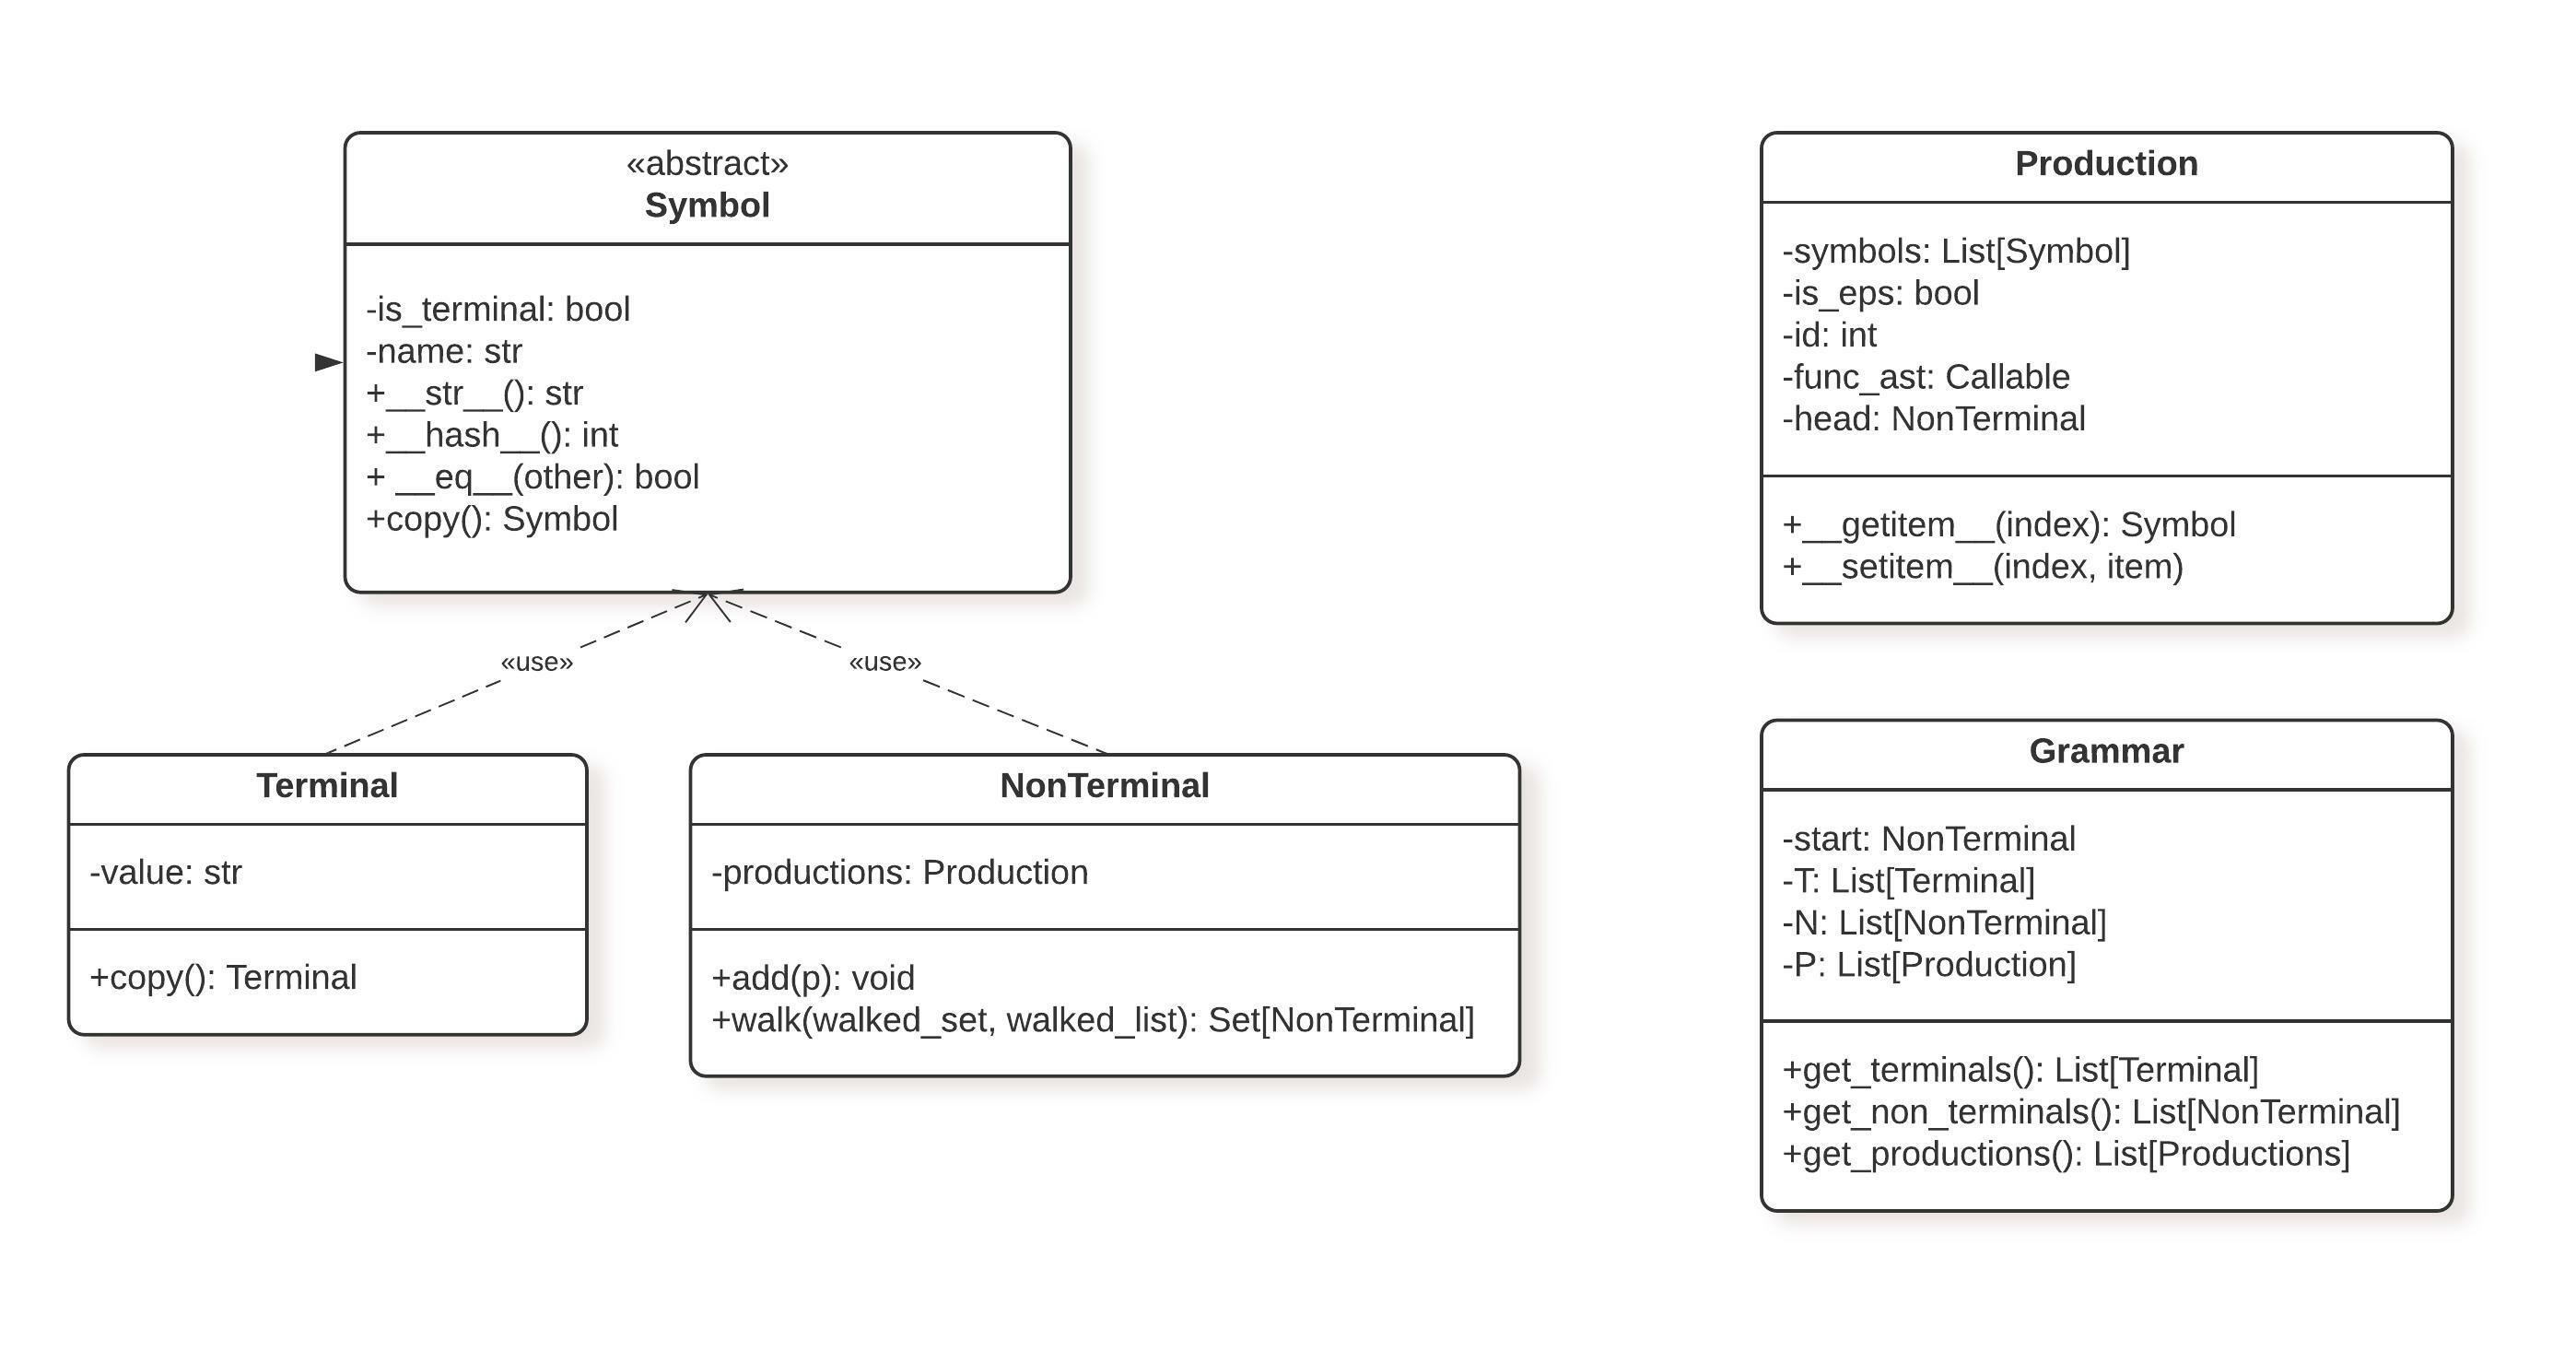
\includegraphics[width=13cm]{./chapters/img/grammar.jpeg}
        \caption{Diagrama de clases del módulo grammar}
\end{figure}

Para inicializar una gramática es necesario tener creado todos los \verb|NonTerminal| con sus producciones agregadas, y se le pasa el \verb|NonTerminal| inicial al constructor de \verb|Grammar|.

Luego de crear dicho submódulo se implementó la gramática en el archivo \verb|bs_grammar.py| de forma que esté accesible para todo el compilador en la variable \verb|GRAMMAR|.

\subsection{Compilador}

El compilador implementado es un transpilador del lenguaje de dominio específico Battle Script hacia Python. Para ello se implementaron las siguientes etapas del proceso de compilación: tokenización, parsing, análisis semántico y generación de código.

\subsection{Tokenizador}

Un Tokenizador, comúnmente llamado Lexer, es un ente encargado de dividir la cadena de texto de entrada del compilador en tokens del alfabeto del lenguaje Battle Script, identificando el tipo del token y envíandolo a la siguiente etapa del proceso de compilación.

Para la implementación del tokenizador fue necesario un sistema de expresiones regulares, una clase para representar un token, así como su tipo y la definición de los tokens del lenguaje, además de la clase propia del tokenizador. 

\subsubsection{Sistema de expresiones regulares}

Una expresión regular es una definición recursiva de un lenguaje donde $a$ es la expresión regular para $L(a) = \{a\}$ y $\epsilon$ es la expresión regular para $L(\epsilon) = \{\epsilon\}$. Si $s$ y $r$ son expresiones regulares entonces:

\begin{itemize}
    \item $(s)|(r)$ es la expresión regular para la unión de lenguajes $L(s) \cup L(r)$
    \item $(s)(r)$ es la expresión regular para la concatenación de lenguajes $L(s)L(r)$
    \item $(s)*$ es la expresión regular para la clausura del lenguaje $L(s)* = \bigcup\limits_{k=0}^{\infty} L(s)^k$
\end{itemize}

Se implementó un sistema de expresiones regulares que admite los siguientes operadores:

\begin{itemize}
    \item $|$ que hace la unión de dos expresiones regulares.
    \item La concatenación de expresiones regulares de la siguiente forma, si $a$ y $b$ son expresiones regulares entonces $ab$ es la expresión de la concatenación.
    \item $*$ que hace la clausura del lenguaje que representa la expresión regular.
    \item $?$ que busca la coincidencia de la expresión regular una vez o ninguna.
    \item $+$ que busca la coincidencia de la expresión regular una o más veces.
    \item $.$ que busca la coincidencia de ninguno o cualquier caracter.
    \item $\setminus$  que permite la inclusión de los operadores anteriores en un expresión regular como un caracter.
\end{itemize}

La gramática para el lenguaje de las expresiones regulares que se implementó es la siguiente:

\begin{verbatim}
    regex = exp 

    exp      = term '|' exp    
            | term

    term     = factor term       
            | factor

    factor   = primary '*'      
            | primary '+'       
            | primary '?'       
            | primary

    primary  = '(' exp ')'
            | '\' CHAR              
            | CHAR
            | '.'
\end{verbatim}

Una expresión regular en el sistema se implementó utilizando la clase \verb|Regex|. Una expresión regular se construye con la cadena de texto que representa el patrón de la expresión regular. Este patrón se compila y se devuelve un Autómata Finito No Determinista (NFA) que se utiliza para los procesos de saber si una cadena pertenece al lenguaje representado por la expresión, o encontrar todas las coincidencias de la expresión en una cadena de texto. 

\begin{verbatim}
class Regex:
        def __init__(self, pattern: str):
            self.pattern : str = pattern
            self.nfa : NFA = self.compile()
    
        def compile(self) -> NFA:
            lex: Lexer = Lexer(self.pattern)
            parser : Parser = Parser(lex)
            tokens : List[Token] = parser()
            handler: Handler = Handler()
            
            nfa_stack : List[NFA]= []
            
            for t in tokens:
                handler.handlers[t.name](t, nfa_stack)
            
            if len(nfa_stack) == 1:
                return nfa_stack.pop() 
            raise Exception("Bad regex!")
    
        def match(self, string: str) -> bool:
            return self.nfa.match(string)
    
        def find_all(self, string: str) -> List[Match]:
            return self.nfa.find_all(string)
\end{verbatim}

El proceso de compilación de una expresión regular es bastante sencillo, se tiene un tokenizador que recorre la cadena y cada vez que encuentra un operador o un caracter devuelve el token correspondiente, si encuentra el operador de escape ($\setminus$) devuelve un token de tipo \verb|CHAR| con el caracter siguiente. El proceso de Parsing consiste en recibir el conjunto de tokens provenientes del tokenizador y llamar al método \verb|exp| que este parsea el no terminal del mismo nombre de la gramática y va parseando el resto de no terminales según corresponda, o sea, se implementó un Parsing Recursivo Descendente.

Luego del proceso de parsing y verificar que la secuencia de tokens es correcta, se recorre la secuencia de tokens y haciendo uso de la clase \verb|Handler| se construye el autómata de la expresión regular. 

La clase \verb|Handler| es la encargada de dado un conjunto de tokens construir el autómata correspondiente, para ello implementa un método para cada operador de la gramática, estos métodos saben construir el autómata que resulta de aplicar la operación a uno, dos o más autómatas según el operador. La clase implementa el algoritmo Thompson's construction para la construcción del autómata.

\begin{itemize}
        \item \textbf{Reconcimiento de un caracter:} el método de la clase \verb|Handler| encargado de construir dicho autómata construye el estado inicial \verb|s0| y el final \verb|s1| y añade la transición con el caracter en cuestión, como se muestra en la figura siguiente:
                \begin{figure}
                        \centering
                        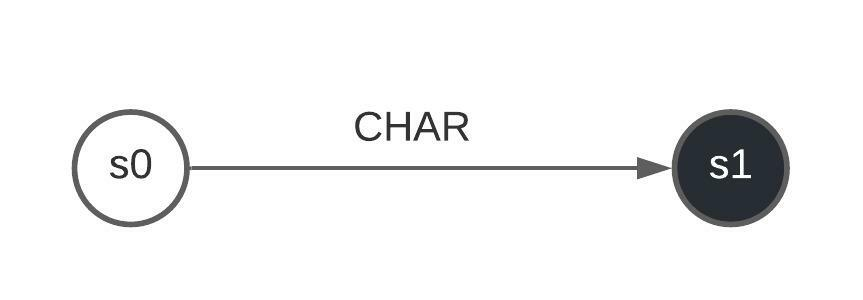
\includegraphics[width=6cm]{./chapters/img/char.jpeg}
                        \caption{Autómata finito no determinista para el reconocimiento de un caracter}
                \end{figure}
        \item \textbf{Operación de Unión:} el método encargado de construir el autómata solo debe los estados iniciales y finales, además añadir $\epsilon$-transiciones desde el estado incial hacia los autómatas y desde los autómatas hacia el estado final.
                \begin{figure}
                        \centering
                        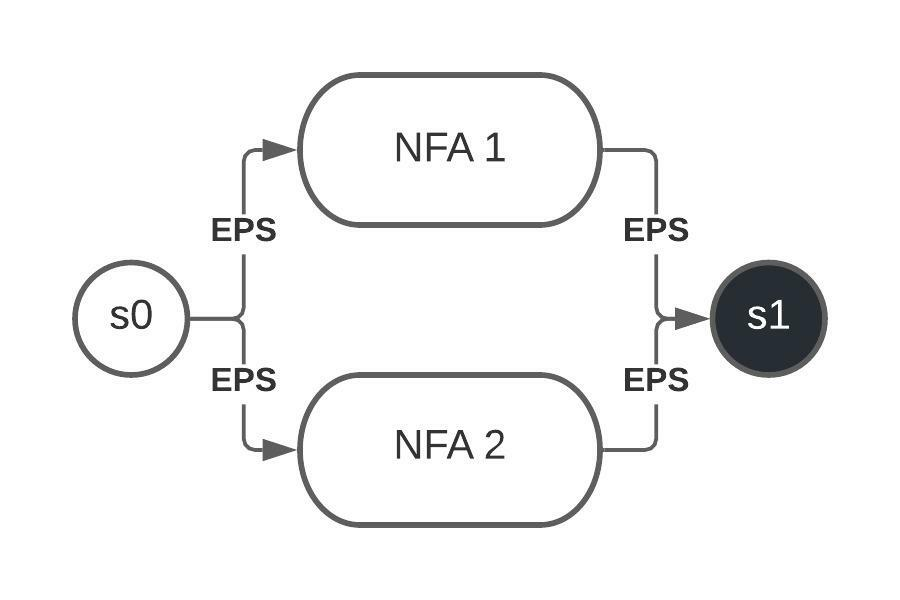
\includegraphics[width=6cm]{./chapters/img/alt.jpeg}
                        \caption{Autómata finito no determinista para el operador unión}
                \end{figure}
        \item \textbf{Operación de Concatenación:} el método encargado de construir el autómata solo debe  añadir una $\epsilon$-transición desde el estado final del primer autómata hacia el estado incial del segundo autómata.
                \begin{figure}
                        \centering
                        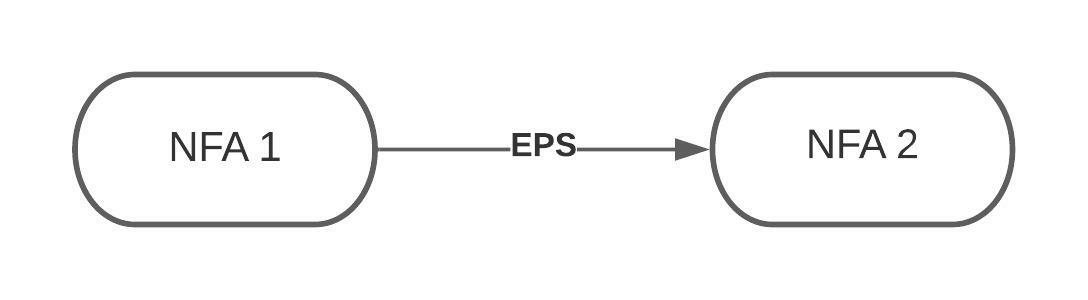
\includegraphics[width=6cm]{./chapters/img/concat.jpeg}
                        \caption{Autómata finito no determinista para el operador concatenación}
                \end{figure}
        \item \textbf{Operación} \verb|*|: el método encargado de construir el autómata solo debe los estados iniciales y finales, además añadir $\epsilon$-transiciones desde el estado incial hacia el autómata y desde el autómata hacia el estado final, así como una desde \verb|s0| hacia \verb|s1| para reconocer la no aparición del patrón, y una transición $\epsilon$ desde el estado final del autómata hacia el inicial para reconocer las repeticiones.
                \begin{figure}
                        \centering
                        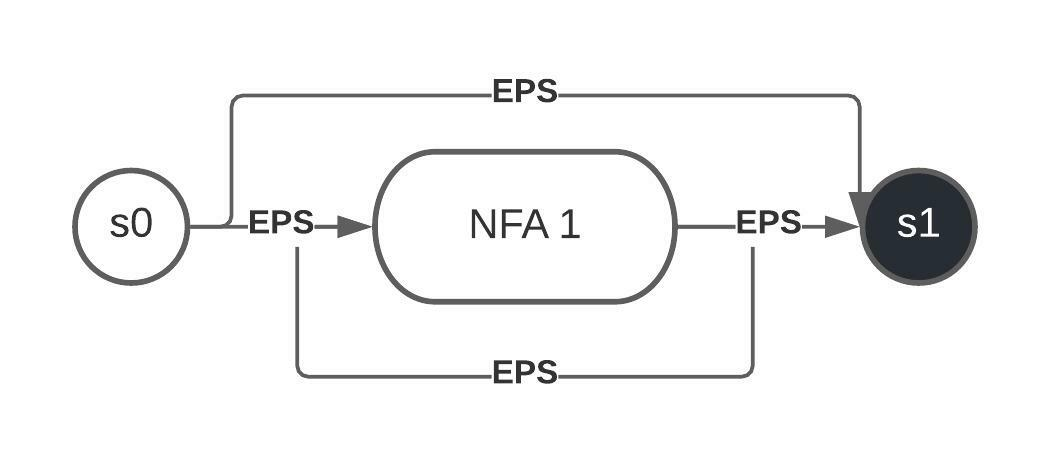
\includegraphics[width=6cm]{./chapters/img/star.jpeg}
                        \caption{Autómata finito no determinista para el operador *}
                \end{figure}
        \item \textbf{Operación} \verb|+|: el método encargado de construir el autómata solo debe los estados iniciales y finales, además añadir $\epsilon$-transiciones desde el estado incial hacia el autómata y desde el autómata hacia el estado final, y una transición $\epsilon$ desde el estado final del autómata hacia el inicial para reconocer las repeticiones.
                \begin{figure}
                        \centering
                        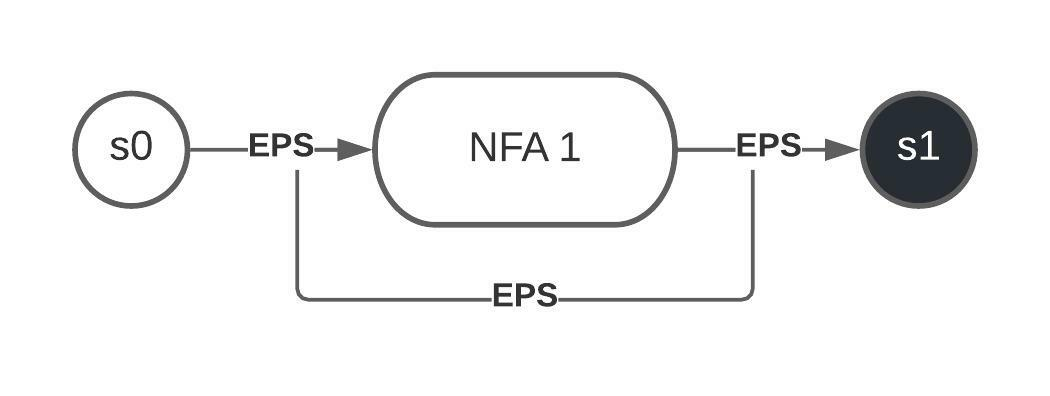
\includegraphics[width=6cm]{./chapters/img/plus.jpeg}
                        \caption{Autómata finito no determinista para el operador +}
                \end{figure}
        \item \textbf{Operación} \verb|.|: el método encargado de construir dicho autómata construye los estados inciales y finales ya añade un transición para cada caracter y añade un $\epsilon$-transición para reconocer la ocurrencia de ningún caracter.
                \begin{figure}
                        \centering
                        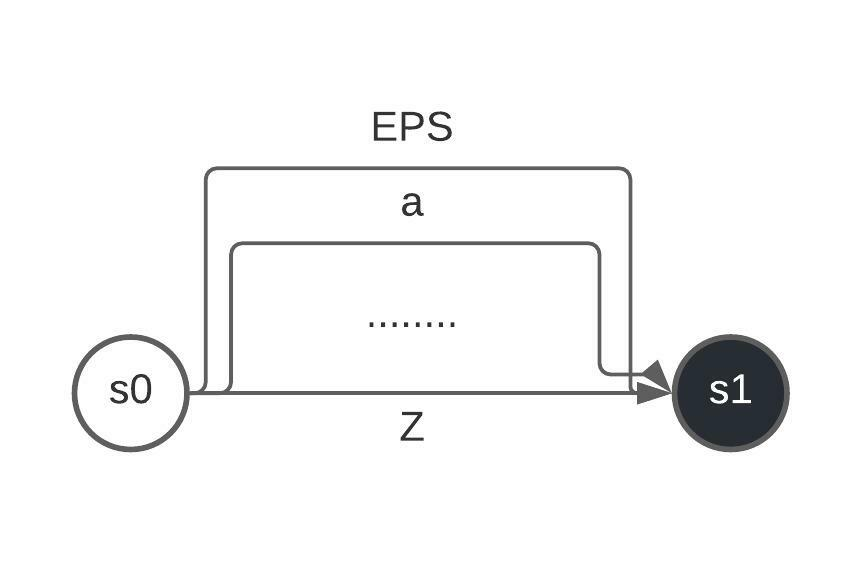
\includegraphics[width=6cm]{./chapters/img/dot.jpeg}
                        \caption{Autómata finito no determinista para el operador .}
                \end{figure}
        \item \textbf{Operación} \verb|?|: el método encargado de construir dicho autómata debe añadir una $\epsilon$-transición desde el estado incial del autómata hacia el estado final del autómata para reconocer la no aparición del patrón.
                \begin{figure}
                        \centering
                        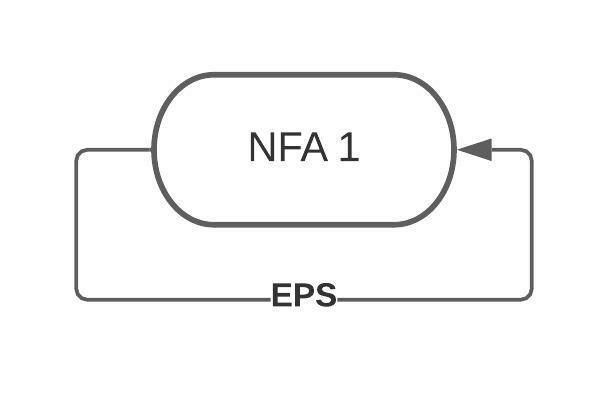
\includegraphics[width=6cm]{./chapters/img/qmark.jpeg}
                        \caption{Autómata finito no determinista para el operador ?}
                \end{figure}
\end{itemize}

Luego que se construye el autómata para una expresión regular  el proceso de compilación ha terminado. 

Entonces, ¿cómo saber si una cadena de texto pertence al alfabeto representado por una expresión regular? Para ello existen varios enfoques entre ellos están:

\begin{itemize}
        \item \textbf{Enfoque inocente o tonto:} utilizando backtracking y revisando los operadores y la cadena. Este enfoque es bien costoso y no aprovecha las potencialidades de los autómatas anteriormente construidos.
        \item \textbf{Enfoque DFA:} se construye un Autómata Finito Determinista (DFA) a partir del no determinista anteriormente construido y se hace una pasada sobre él. Este enfoque es correcto, pero implica un procesamiento extra para construir el DFA.
        \item \textbf{Enfoque NFA:} este es el enfoque implementado en el proyecto en el método \verb|match| de una \verb|Regex|, que consiste en hacer una pasada sobre el autómata no determinista y revisar si coincide la cadena, pero el no determinismo trae un problema consigo, es que en un estado \verb|x| no se sabe con total seguridad que transición aplicar. Para ello, la propuesta es ejecutar las transiciones a la vez y ver si por alguna se llega al estado final. Esto hace que el tiempo de reconocimiento sea lineal respecto al tamaño de la cadena de entrada.
\end{itemize}

Entonces, ¿cómo encontrar todas las coincidencias de un patrón dentro de una cadena de texto?. Para ello se modificó el método anterior y cada vez que no se podía continuar  porque venía un caracter desconocido para la expresión regular se volvía al estado inicial. Además en cada posición se revisa si se ha llegado al estado final, se devuelve la coincidencia y se vuelve al estado inicial. Este procedimiento se implementó en método \verb|find_all| de las \verb|Regex|. Este procedimiento es lineal con respecto al tamaño de la cadena.

Luego de implementado el sistema de expresiones regulares se implementó la clase \verb|Token| y el enum \verb|TokenType|.

\subsubsection{Token y TokenType}

Un token en el proyecto se representa con la clase \verb|Token| que tiene la siguiente implementación. La propiedad \verb|regex| almacena la expresión regular que coincide con el token, la propiedad \verb|name| representa el nombre del tipo de token, la propiedad \verb|lexeme| almacena la cadena de texto que se extrajo de la cadena de entrada como token, es decir, si se tiene un token \verb|t| entonces \verb|t.regex.match(t.lexeme)| es verdadero. Además, un token almacena donde comienza y termina \verb|lexeme| en la cadena de entrada.

\begin{verbatim}
class Token:
        @propertyclass Token:
        @property
        def regex(self) -> Regex:
            return self.type.value[0]
    
        @property
        def name(self) -> str:
            return self.type.value[1]
            
        def __init__(self, token_type: TokenType, lexeme: str, start: int, end: int):
            self.type: TokenType = token_type
            self.lexeme: str = lexeme
            self.start: int = start
            self.end: int = end
        
    
        @property
        def name(self) -> str:
            return self.type.value[1]
            
        def __init__(self, token_type: TokenType, lexeme: str, start: int, end: int):
            self.type: TokenType = token_type
            self.lexeme: str = lexeme
            self.start: int = start
            self.end: int = end
        
\end{verbatim}

El tipo de los tokens se definió utilizando el enum \verb|TokenType| que representa la expresión regular que lo representa y el nombre del token, por ejemplo: para el token que representa la palabra reservada \verb|eq| el \verb|TokenType| correspondiente es \verb|Eq = (Regex("eq"), "eq")|

\subsubsection{Algoritmo del tokenizador}

El algoritmo del tokenizador sigue la siguiente idea general, se le asocia a cada token de la gramática un nivel de precedencia que representa cuán relevante es un token sobre otro. Por ejemplo si se tienen los siguientes: \verb|Token((Regex("eq"), "eq"), "eq", 1, 2)| y \texttt{Token((Regex("(a|b|....|Z)+"), "NAME"), 'eq', 1, 2)} donde el primer token tiene precedencia 1 y el segundo tiene 2, entonces el token más relevante es el primero. Entonces, se tiene una lista \verb|tokens| y se recorre la lista de tokens de la gramática y a cada uno se le piden todas coincidencias en la cadena de entrada. Luego se recorren las posiciones \verb|i| de la cadena de entrada, y se añade a \verb|tokens| aquel token que comience en \verb|i| y tenga menor precedencia.

\begin{verbatim}
class Tokenizer:
    def __call__(self, bs_content_file: str) -> Iterable[Token]:
        tokens: List[Token] = []

        matches = {}
        for token_def in TOKENS:
            matches[token_def] = token_def.type.value[0].find_all(bs_content_file)
        
        i = 0
        while i < len(bs_content_file):
            token_in_i: List[Tuple[TokenDefinition, Match]] = []

            # Get all matches
            for k, v in matches.items():
                for t in v:
                    if t.start == i:
                        token_in_i.append((k, t))
                    
            # Get match with highest precedence
            if len(token_in_i):
                token_in_i = sorted(token_in_i, key=lambda tup: tup[0].precendece)
                token = Token(token_in_i[0][0], \
                                token_in_i[0][1].value,\
                                token_in_i[0][1].start,\
                                token_in_i[0][1].end)
                tokens.append(token)    
                i = token.end

            i += 1
        return deque(tokens)
\end{verbatim}

Este algoritmo tiene complejidad temporal $O(n*m)$ donde $m$ es la cantidad de tokens, y $n$ el tamaño de la cadena de entrada.

\subsection{Parser}

\subsubsection{Construcci\'on del Parser}

El parser implementado es un parser $LR(1)$ can\'onico, el cual es un parser $LR(k)$ con $k = 1$, es decir, con un solo terminal de anticipación. Una característica especial de este parser es que cualquier gramática $LR(k)$ con $k>1$ puede transformarse en una gramática $LR(1)$. Para la implementación se definieron las clases \verb|Item| e \verb|ItemLR1| que representan la definici\'on de Item LR(0) e Item LR(1).

La clase \verb|Item| tiene como atributos una producci\'on y un \'indice tal que los s\'imbolos en las posiciones menores que el \'indice son los s\'imbolos de la producci\'on que se han detectado y los s\'imbolos en las posiciones mayores o igual al \'indice son los s\'imbolos de la producci\'on que faltan por ver.

Como se dijo anteriormente la clase \verb|ItemmLR1| es la definici\'on de un item LR(1). Obs\'ervese que esta hereda de \verb|Item| y adem\'as se agregan como atributos adicionales el \verb|lookahead|, un string que representa al item y un valor de hash calculado a partir de este string. Adem\'as se implementan las funciones de \verb|__hash__| y \verb|__eq__|. 

Adem\'as se implement\'o la clase \verb|State| que representa un estado del aut\'omata LR(1). Un estado tiene los siguientes atributos:

\begin{itemize}
	\item \verb|kernel| que es una lista de items LR(1) que son el kernel del estado.
	\item \verb|string| un cadena que representa al estado, que no es m\'as que la concatenaci\'on de los items kernel del estado delimitados por el caracter $|$.
	\item \verb|items| que es el conjunto de items del estado (de ah\'i la necesidad de implementar la funci\'on \verb|__hash__| para la clase \verb|ItemLR1|).
	\item \verb|nexts| es un diccionario tal que las llaves son los s\'imbolos que pueden venir a continuaci\'on dado que el parser se encuentra en dicho estado; y el valor asociado al s\'imbolo es el estado al que se mueve el parser si se detecta dicho s\'imbolo.
	\item \verb|expected_symbols| es un diccionario tal que las llaves son los s\'imbolos que pueden venir a continuaci\'on dado que el parser se encuentra en dicho estado; y el valor asociado al s\'imbolo es un conjunto de items del estado que tienen a dicho s\'imbolo en la posici\'on que marca su \'indice respectivo.
	\item \verb|number| que es el n\'umero correspondiente al estado.
\end{itemize} 

Esta clase tiene definida, entre otras, tres funciones interesantes: \verb|add_item(self, item: ItemLR1)|, \verb|build(self, initial_items)| y \verb|go_to(self, sym: Symbol, states_dict, state_list, q: deque,| \verb| initial_items)|. La primera a\~{n}ade un item LR(1) al conjunto de items del estado. La segunda se utiliza para construir el estado a partir de los items kernel del estado y los items iniciales de la gram\'atica(los que tienen su \'indice en 0). La idea detr\'as de este segundo m\'etodo es crear una cola a partir de los items kernel, luego mientras la cola no este vac\'ia se extrae el primer item de la cola. Si el s\'imbolo en la posici\'on que indica el \'indice es un no terminal se computan todos los items no kernel que este item genera y por cada uno de estos se comprueba si ya pertenece al conjunto de items del estado. En caso de no estarlo se a\~{n}ade el item al conjunto de items y a la cola de items. 

La tercera funci\'on se utiliza para computar todas las transiciones desde el estado actual hacia otro estado dado un s\'imbolo determinado. La idea seguida para esta funci\'on es por cada uno de los items que tienen al s\'imbolo en la posici\'on que indica su respectivo \'indice, generar un nuevo item con los mismos atributos que el item original excepto por el \'indice, que ser\'a el del original aumentado en 1. F\'ijese que los nuevos items generados indican que ya se vio el s\'imbolo analizado en sus respectivas producciones. Estos nuevos items se a\~{n}aden a una lista, con la cual se crea un nuevo estado a partir de dicha lista. O sea, dicha lista es el kernel del nuevo estado. Luego se comprueba si este nuevo estado ya fue generado. Si no lo ha sido entonces se construye el nuevo estado por completo. Finalmente se a\~{n}ade la transici\'on.

Luego se tiene la clase \verb|Automaton| la cual se instancia con una gram\'atica y tiene definida la funci\'on \verb|build(self)|; la cual construye un aut\'omata LR(1) a partir de la gram\'atica. Esta funci\'on devuelve una lista de estados y las transiciones vienen dadas por el diccionario \verb|nexts| que cada estado tiene como atributo. En este m\'etodo primero se crea un s\'imbolo inicial y se la a\~{n}ade una producci\'on con el s\'imbolo inicial de la gram\'atica. Luego por cada una de las producciones se generan los items iniciales. Luego se crea el estado inicial y a partir de este se van generando el resto de los estados utilizando una cola de estados, que se inicializa con el estado inicial, y la funci\'on \verb|go_to| de cada estado.  Mientras la cola no este vacia se extrae el primer estado de la misma, se llama a la funci\'on \verb|go_to| con cada uno de los posibles s\'imbolos y cada vez que se encuentre un estado nuevo se a\~{nade} a la cola. Los nuevos estados se van guardando en una lista que es la que devuelve el m\'etodo.

Por \'ultimo tenemos la clase \verb|TableActionGoTo|, la cual se instancia a partir de una gram\'atica y tiene un m\'etodo \verb|build(self, path: str)| la cual construye las tablas ``Action'' y ``GoTo'' y las guarda como objetos .json en la direcci\'on especificada. Ambas tablas las representaremos como listas de diccionarios, tal que el elemento $i$ de cada lista ser\'a un diccionario correspondiente al estado $i$ del aut\'omata. La lista \verb|action| representar\'a la tabla ``Action'' y la lista \verb|go_to| representar\'a la tabla ``GoTo''.

Entonces por cada estado se crean dos diccionarios: \verb|state_action| y \verb|state_go_to| y se analizan cada una de sus posibles transiciones. Si el s\'imbolo con el que se hace la transici\'on hacia otro estado es un terminal entonces, se agrega al diccionario \verb|state_action| el s\'imbolo como llave y una tupla de dos elementos como su valor correspondiente, de tal forma que el primer elemento de dicha tupla es el car\'acter 'S', que indica que la acci\'on a hacer es Shift, y el segundo elemento es el n\'umero del estado al que lleva la transici\'on. Si por el contrario el s\'imbolo es un no terminal se a\~{n}aden como llave y valor respectivamente el s\'imbolo y el n\'umero del estado al que lleva la transici\'on en el diccionario \verb|state_go_to|. Luego se analizan todos los items del estado cuya producci\'on ya fue vista por completo y si existe un par de items con igual lookahead se reporta la existencia de un conflicto Reduce - Reduce.

Por cada lookahead y su respectivo item detectados anteriormente, se chequea si el lookahead aparece entre las llaves del diccionario \verb|state_action| y de ser as\'i entonces ocurre un conflicto Shift-Reduce y se reporta el mismo. En caso contrario se a\~{n}ade al diccionario \verb|state_action| el lookahead como llave y como su valor asociado una tupla de dos elementos, tal que el primer elemento es el car\'acter 'R', que indica que hay que hacer Reduce, y el segundo elemento es el id de la producci\'on que se debe reducir. Si el lookahead detectado es el s\'imbolo especial '\$' y adem\'as la parte izquierda del item correspondiente es el s\'imbolo 'S' definido como el inicial, entonces la cadena es v\'alida y se a\~{n}ade al diccionario \verb|state_action| dicho s\'imbolo como llave y como su valor correspondiente una tupla con un solo elemento : la cadena 'OK'. 

Luego de todos estos an\'alisis sobre el estado se a\~{n}aden los diccionarios \verb|state_action| y \verb|state_go_to| a las listas \verb|action| y \verb|go_to| respectivamente. Cuando se terminen de analizar todos los estados estas listas se guardan en sendos archivos de tipo json en la direcci\'on especificada.

\subsubsection{AST y \'Arbol de derivaci\'on}
Para la construcci\'on del AST durante el proceso de parsing se implementaron las definiciones de sus nodos y de algunos nodos del \'arbol de derivaci\'on, para facilitar este proceso. Los nodos del AST heredan de forma indirecta de la clase abstracta \verb|Node|, dividi\'endose en instrucciones y expresiones, excepto por los siguientes nodos que heredan directamente de \verb|Node|:

\begin{itemize}
	\item \verb|BSFile|: Nodo ra\'iz del AST.
	\item \verb|AttrDef|: Definici\'on de atributo de una clase.  
	\item \verb|ClassDef|: Definici\'on de una clase.
\end{itemize}

Los nodos instrucciones son los siguientes:

\begin{itemize}
	\item \verb|FuncDef|: Definici\'on de funci\'on.
	\item \verb|If|: Instrucci\'on \textbf{if}. 
	\item \verb|Branch|: Lista de instrucciones \textbf{if} y una instrucci\'on \textbf{else}
	\item \verb|WhileDef|: Instrucci\'on \textbf{while}
	\item \verb|Decl|: Declaraci\'on de variable.
	\item \verb|Assign|: Asignaci\'on de variable. 
	\item \verb|Return|: Instrucci\'on \textbf{return}.
	\item \verb|Break|: Instrucci\'on \textbf{break}.
	\item \verb|Continue|: Instrucci\'on \textbf{continue}.
\end{itemize}

Los nodos expresiones son los siguientes:

\begin{itemize}
	\item \verb|BinaryExpression|: Expresi\'on binaria.
	\item \verb|AritmeticBinaryExpression|: Expresi\'on binaria que solo se puede realizar entre dos n\'umeros.
	\item \verb|TernaryExpression|: Expresi\'on ternaria
	\item \verb|Inversion|: Expresi\'on que es la negaci\'on de otra expresi\'on.
	\item \verb|Primary|: Engloba tanto el llamado a una funci\'on, como la acci\'on de referirse a un atributo de la clase (incluyendo las funciones de dicha clase).
	\item \verb|Variable|: Variable.
	\item \verb|Number|: N\'umero
	\item \verb|Bool|: Expresi\'on booleana
	\item \verb|MyNone|: Expresi\'on None
	\item \verb|MyList|: Lista
	\item \verb|PExpression|: Expresi\'on entre par\'entesis
\end{itemize}

El resto de clases implementadas en este m\'odulo corresponden a los nodos del \'arbol de derivaci\'on, los cuales son utilizados para construir los nodos anteriormente mencionados.

Para construir al AST durante el proceso de parsing se atributaron algunas derivaciones de la gram\'atica, utilizando las funciones implementadas en el m\'odulo src.language.parser.engine\_ast.

\subsubsection{Parseo de una cadena}

Para esto se implement\'o la clase \verb|Parser|, la cual se instancia con una gram\'atica y las tablas de ``Action'' y ``GoTo''. En esta clase se implement\'o la funci\'on \verb|parse|, la cual recibe una cola de tokens y de ser una cadena sint\'acticamente correcta, devuelve el AST generado a partir de la cadena. Primeramente se a\~{n}ade un token especial que se considera como el toquen final de la secuencia y se definen tres pilas:

\begin{itemize}
	\item \verb|tokens_stack|: En esta se van a ir guardando los lexemas de los tokens vistos.
	\item \verb|states_stack|: En esta se van a ir guardando los estados por los que se ha transitado hasta el momento.
	\item \verb|nodes|: En esta se van a ir guardando los nodos del AST y el \'arbol de derivaci\'on. De tal forma que al final del proceso de parsing, en esta solo quede la ra\'iz del AST.
\end{itemize}

Entonces mientras queden tokens por ver de la secuencia, se toma el primer token de la misma y se cargan las acciones del estado actual (el que est\'a en el tope de la pila de estados). Si no existe ninguna acci\'on con dicho token hacia otro estado, entonces se reporta que se detect\'o un token inesperado en la secuencia. Pasado este punto se consulta por la acci\'on que se debe realizar. 

Si la acci\'on es 'OK' es porque la cadena es v\'alida y se retorna el objeto en la posici\'on 0 de la pila \verb|nodes| (el AST). Si la acci\'on es hacer Shift se a\~{n}ade el estado a la pila de estados, se a\~{n}ade el lexema del token a la pila de los tokens y se saca el mismo de la secuencia.

Si lo que toca es hacer Reduce, entonces se obtiene la producci\'on con la que se va a reducir y si adem\'as la producci\'on es atributada, o sea si esta producci\'on tiene asociada una funci\'on que construye un nodo del AST o del \'arbol de derivaci\'on, se llama a esta funci\'on pas\'andole como argumentos la pila de tokens y la pila de nodos. Estas funciones son las que modifican la pila de nodos. Cada una de ellas extrae o no un determinado n\'umero de nodos de la pila de nodos y agrega un nodo nuevo a la pila de nodos. Luego se extraen de la pila de tokens una cantidad de elementos igual a la longitud de la parte derecha de la producci\'on que se reduce. De igual forma se hace con la pila de estados. 

Entonces con el estado que queda en el tope de la pila se cargan utilizando la tabla ``GoTo'' las transiciones que se pueden hacer con no terminales en dicho estado. Si no existen transiciones en dicho estado con el no terminal que es parte izquierda de la producci\'on que se redujo, entonces se lanza un error indicando que la secuencia de tokens es inv\'alida. En caso contrario se a\~{n}ade el no terminal a la pila de tokens y se a\~{n}ade el estado al que se avanza con dicho token a la pila de estados.

\subsection{An\'alisis Sem\'antico}
\subsubsection{Definiendo tipos}
Para implementar nuevos tipos en el lenguaje se implement\'o una clase \verb|Type| en la que cada clase del lenguaje ser\'a una instancia de esta.
 
  \verb|Type| consta de los siguientes atributos y m\'etodos 
  \begin{itemize}
  \item Atributos
  \begin{itemize}
  \item \verb|name|: Nombre de la clase o nuevo tipo
  
  \item \verb|parent|: Tipo inmediato del cuál hereda este tipo
  
  \item \verb|context|: Contexto en que se encuentran todos los atributos y métodos de este tipo. 
  
  \item \verb|def_context|: Contexto en el que se encuentra este tipo
  \end{itemize}
  
  \item M\'etodos
  \begin{itemize}  
  \item \verb|define_attribute|: Define un atributo de la clase.
  
  \item \verb|define_method|: Define un m\'etodo de la clase.
  
  \item \verb|is_attribute|: Revisa si el atributo existe.
  
  \item \verb|check_method|: Revisa que el método esté bien definido a partir de los atributos
  
  \item \verb|is_method|: Revisa si el m\'etodo existe.
  
  \item \verb|is_child|: Revisa si el nombre dado es padre del tipo.
  \end{itemize}
  \end{itemize}
  Estos métodos en su mayoría se apoyan en funciones del contexto para definir y revisar atributos dentro del contexto del tipo creado.
  
  Los tipos admitidos en el lenguaje son los siguientes:
  
  \begin{itemize}
  	\item \verb|number|: Que engloba a los n\'umeros.
  	\item \verb|bool|: Que engloba a las expresiones booleanas
  	\item \verb|List|: Que engloba a las listas. Una lista cuenta con dos funciones: \verb|append| y \verb|remove| para a\~{n}adir y remover elementos de la misma respectivamente.
  	\item Todos los tipos descritos durante la explicaci\'on de la simulaci\'on con sus respectivos m\'etodos y atributos. Aqu\'i vale aclarar que de estos los \'unicos tipos instanciables son \verb|LandMap| y \verb|Simulator|.
  	\item Los nuevos tipos definidos por el usuario que se explican a continuaci\'on (que tambi\'en son instanciables).
  \end{itemize}
  
  En nuestro lenguaje lo primero que se hace una vez que se crea un tipo es revisar si este tiene un padre. En este lenguaje todos los tipos definidos por el usuario deben heredar de \verb|LandUnit|, \verb|NavalUnit| o \verb|StaticObject| en caso contrario se lanzará una excepción. Una vez que se conoce cuál es la clase de la cuál se hereda, se procede a copiar los atributos y tipos definidos en la clase padre. Las funciones heredadas pueden ser modificadas una única vez durante la definición de la clase. Además cada función tiene en su contexto definida la función \verb|super()| que devuelve el tipo de la clase padre y de esta forma se puede llamar a la definición de la función en la clase padre directamente.
  
  Adem\'as se tienen como funciones built-in del lenguaje las funciones \verb|build_random_map| y \verb|print|.
  
  La función \verb|build_random_map| es una función built-in que devuelve una instancia de \verb|LandMap| y recibe como parámetros un número
  real entre 0 y 1 que indica el porcentaje de casillas de tierra que se desea tenga el mapa, y dos enteros
  que indican el número de filas y de columnas que se desea tenga el mapa.
  
  La funci\'on \verb|print| recibe un argumento e imprime en consola dicho argumento.

\subsubsection{Context}
Para definir el contexto en el que se escribe un programa con el lenguaje, se implement\'o la clase \verb|Context|, esta cuenta con los siguientes atributos y m\'etodos 
\begin{itemize}
\item Atributos
\begin{itemize}
\item \verb|name|: Nombre del contexto 

\item \verb|father|: Contexto padre de este contexto

\item \verb|children|: Contextos hijos de este contexto

\item \verb|_var_context|: Variables del contexto. 

\item \verb|_func_context|: Funciones del contexto

\item \verb|_type_context|: Tipos definidos en el contexto

\item \verb|If|: Cantidad de sentencias \verb|If| definidas en el contexto

\item \verb|Else|: Cantidad de sentencias \verb|Else| definidas en el contexto

\item \verb|While|: Cantidad de sentencias \verb|While| definidas en el contexto
\end{itemize}

\item M\'etodos
\begin{itemize}
\item \verb|check_var|: Revisa si la variable est\'a definida en el contexto.

	\item \verb|check_var_type|: Revisa que la variable est\'e definida en el contexto y el tipo corresponda con el tipo de la variable.
	
	\item \verb|check_func|: Revisa que la funci\'on est\'e definida.
	
	\item \verb|check_func_args|: Revisa si la funci\'on est\'a definida y los tipos de los argumentos coinciden con los tipos de la funci\'on.
	
	\item \verb|get_type|: Devuelve el tipo de una variable en el contexto.
	
	\item \verb|define_var|: Si la variable no existe en el contexto, la crea. 
	
	\item \verb|define_func|: Define la funci\'on si no existe en el contexto. Una función solo puede definirse una vez. En caso de funciones heredadas estas pueden re-definirse una única vez. Cuando se crea una función se crea además un contexto, el contexto que ella define que viene a ser el cuerpo del método.
	
	\item \verb|create_child_context|: Crea un contexto hijo.
	
	\item \verb|create_type|: Crea un nuevo tipo en el contexto. Una vez que se crea un tipo se define una función dentro del contexto donde se crea el tipo y con el mismo nombre de este, la cual será el constructor de la clase. Además, una clase también define un contexto, donde estarán todos sus atributos. Se tiene además una propiedad que dice si el tipo es accesible. Por defecto todos los tipos son accesibles. Si un tipo no es accesible no se podrá instanciar pues no tendrá definida una función constructor. Usualmente esta propiedad es para algunos tipos built-in, por ejemplo \verb|number|, pues no tendría sentido hacer: \verb|number a = number();|.
	
	\item \verb|get_return_type|: Devuelve el tipo de retorno de una funci\'on si esta est\'a definida en el contexto.
	
	\item \verb|get_type_object|: Devuelve la clase a la que pertenece un objeto dado. 
	
	\item \verb|is_type_defined|: Analiza si el tipo est\'a definido.
	
	\item \verb|is_context_father|: Revisa si el contexto dado es ancestro de este contexto.
	
	\item \verb|get_context_father|: Devuelve el contexto dado si es ancestro de este contexto.
	
	\item \verb|is_in_while_context|: Revisa si el contexto actual está definido dentro de un contexto while. De esta forma \verb|break| y \verb|continue| no pueden ser usadas si no están dentro de un bucle.
	
	\item \verb|is_in_func_context|: Revisa si el contexto actual está definido dentro de un contexto función pues sería incorrecto usar una expresión de tipo \verb|return| fuera de un método. 
	
	\item \verb|check_type|: A este método se le pasan dos tipos y comprueba que el primero sea ancestro del segundo.

	
\end{itemize}

\end{itemize}

Se definió \verb|Type| como tipo genérico, que no viene a ser un tipo en sí, es más bien una palabra reservada que significa que puede ser sustituida por cualquier tipo existente.

\subsubsection{Pasadas por el AST}
Para verificar la correcci\'on de la sem\'antica se implement\'o el patr\'on \verb|Visitor| que visitar\'a el \'arbol de sintaxis abstracta en cuatro pasadas distintas
\begin{itemize}
\item \verb|Type_Collector|: Es la primera pasada con el patr\'on \verb|Visitor| en este se recogen todos los tipos que se van a definir, para crearlos en el contexto. Además se revisa que los tipos que se crearon sean hijos de  \verb|LandUnit|, \verb|NavalUnit| o \verb|StaticObject| en caso contrario lanza una excepción. Se guardarán además el contexto de que define la clase, el contexto donde se define la clase y el contexto que define el constructor de la misma.

\item \verb|Type_Builder|: Es la segunda pasada con el patr\'on, se toman todos los tipos que se definieron anteriormente y se definen sus m\'etodos y atributos. Se guarda además el contexto que define cada función cuando se crea.

\item \verb|Type_Context|: Es la tercera pasada del visitor, se visita cada nodo para definir en qu\'e contexto est\'a. Para esto se usa el atributo \verb|current_context| en el cual se guarda el contexto que se está visitando actualmente, actualizándose cada vez que se pasa por un nodo que define un contexto (clases, funciones, condicionales o bucles) y volviendo al valor anterior una vez que se termina ese camino del \'arbol de sintaxis abstracta. 

\item \verb|Type_Checker|: Es la cuarta pasada con el patr\'on, en esta se revisan que los tipos de cada expresi\'on no entren en contradicci\'on. Para esto se revisa en los contextos donde se encuentran los nodos y se utilizan las funciones de la clase \verb|Context|. Se chequea adem\'as que expresiones de \verb|return| solo ocurran dentro de una función y expresiones como \verb|break| y \verb|continue| estén siempre dentro de un bucle.


\end{itemize}

\subsection{Generaci\'on de c\'odigo}

Para la generaci\'on de c\'odigo se parte de la rai\'z del AST y haciendo uso del patr\'on ``Visitor'' se visitan cada uno de los nodos del AST. El c\'odigo generado es una cadena en c\'odigo Python, de tal forma que se importan todos los m\'odulos necesarios para realizar una simulaci\'on y el c\'odigo Python generado es equivalente a lo que el usuario program\'o en nuestro lenguaje. El c\'odigo referente a este apartado se encuentra en el m\'odulo src.language.code\_generation.code\_genration. En este aparece implementada la clase \verb|CodeGenerate|, la cual tiene como atributos un \verb|StringIO|, un entero que lleva la cantidad de tabuladores para generar el c\'odigo Python correspondiente y un diccionario que traduce algunos de los s\'imbolos de nuestro lenguaje a s\'imbolos en c\'odigo Python. Adem\'as para cada uno de los nodos del AST se implement\'o la funci\'on \verb|visit|. 

Un dato interesante es que para los nodos de tipo \verb|ClassDef| y los nodos de tipo \verb|Statement|, su m\'etodo \verb|visit| correspondiente escribe su c\'odigo correspondiente en el atributo \verb|StringIO| de la clase. Para los nodos de tipo \verb|Expression| se retorna su c\'odigo correspondiente. Esto se hace as\'i dado que en Python casi todo es una instrucci\'on y muchas de estas dependen de expresiones. En el m\'etodo \verb|visit| correspondiente al nodo \verb|BSFile| se escriben todas las importaciones de los m\'odulos necesarios para correr una simulaci\'on; y la cadena del c\'odigo transpilado a Python es la que devuelve este m\'etodo, que devuelve el valor del atributo de tipo \verb|StringIO| de la clase \verb|CodeGenerator|. 

